  \section[OpenStack]{OpenStack : projet, logiciel et utilisation}

  \subsection[OpenStack]{Présentation du projet et du logiciel}

  \begin{frame}
    \frametitle{Historique}
    \begin{itemize}
      \item Démarrage en 2010
      \item Objectif : construire le Cloud Operating System libre
      \item Fusion de deux projets de Rackspace (Storage) et de la NASA (Compute)
      \item Développé en Python et distribué sous licence Apache 2.0
      \item Les dernières releases jusqu'à aujourd'hui :
      \begin{itemize}
        \item Juno (2014.2)
        \item Kilo (2015.1)
        \item Liberty (2015.2)
        \item Mitaka (2016.1)
        \item Newton (2016.2)
        \item Ocata (2017.1)
      \end{itemize}
    \end{itemize}
  \end{frame}

  \begin{frame}
    \frametitle{Les 4 Opens}
    \begin{itemize}
      \item Open Source
      \item Open Design
      \item Open Development
      \item Open Community
    \end{itemize}
  \end{frame}

  \begin{frame}
    \frametitle{Vue haut niveau}
    \includegraphics[width=\textwidth]{images/architecture-simple.jpg}
  \end{frame}

  \begin{frame}
    \frametitle{Les différents sous-projets principaux}
    \begin{itemize}
      \item OpenStack est composé d'un ensemble de briques :
      \begin{itemize}
        \item OpenStack Compute - Nova
        \item OpenStack Block Storage - Cinder
        \item OpenStack Networking - Neutron
        \item OpenStack Image Service - Glance
        \item OpenStack Identity Service - Keystone
        \item OpenStack Telemetry - Ceilometer
        \item OpenStack Orchestration - Heat
        \item OpenStack Dashboard - Horizon
        \item OpenStack (Object) Storage - Swift
        \item et beaucoup d'autres...
      \end{itemize}
    \end{itemize}
  \end{frame}

  \begin{frame}
    \frametitle{Implémentation}
    \begin{itemize}
      \item Chaque brique est découpée en plusieurs services
      \item Ex. avec nova:
        \begin{itemize}
          \item nova-api
          \item nova-compute
          \item nova-scheduler
          \item nova-conductor
          \item etc.
        \end{itemize}
      \item Communication entre les services : AMQP (souvent RabbitMQ)
      \item Base de données : relationnelle SQL (souvent MySQL ou MariaDB)
      \item Neutron utilise pour le réseau : OpenVSwitch
      \item En général : réutilisation de composants existants
      \item Tout est développé en Python (Django pour la partie web)
      \item APIs supportées : OpenStack et équivalent Amazon
      \item Multi tenancy
    \end{itemize}
  \end{frame}

  \subsection[Utilisation]{Utiliser OpenStack}

  \begin{frame}
    \frametitle{Le principe}
    \begin{itemize}
      \item Les APIs sont le principal atout d'OpenStack
      \item Toutes les fonctionnalités sont accessibles par l'API
      \item Les clients (y compris Horizon) utilisent l'API
      \item Des crédentials sont nécessaires
      \begin{itemize}
        \item API OpenStack : utilisateur + mot de passe + tenant
        \item API AWS : access key ID + secret access key
      \end{itemize}
    \end{itemize}
  \end{frame}

  \begin{frame}
    \frametitle{Les APIs OpenStack}
    \begin{itemize}
      \item Chaque service OpenStack a sa propre API
      \item Chaque API est versionnée, la rétro-compatibilité est assurée
      \item Toutes les APIs sont HTTP REST
      \item Certains services sont aussi accessibles via une API différente compatible AWS
      \item http://developer.openstack.org/api-ref.html
    \end{itemize}
  \end{frame}

  \begin{frame}
    \frametitle{Authentification et catalogue de service}
    \begin{itemize}
      \item Avant tout appel a un des services par l'API, il faut s'identifier
      \item Récupération d'un jeton (token)
      \item Récupération du catalogue de services
      \item Pour chaque service, récupération d'un ou plusieurs endpoints HTTP (API)
    \end{itemize}
  \end{frame}

  \begin{frame}
    \frametitle{Accès aux APIs}
    \begin{itemize}
      \item Direct, en HTTP, via des outils comme curl
      \item Avec une bibliothèque
      \begin{itemize}
        \item OpenStack SDK (python)
        \item Shade (python)
        \item Les librairies python-client de chaque projet
        \item D'autres implémentations pour d'autres langages (exemple : jclouds)
      \end{itemize}
      \item Avec les clients officiels en ligne de commande
      \item Avec Horizon
      \item http://docs.openstack.org/user-guide/sdk-overview.html
    \end{itemize}
  \end{frame}

  \begin{frame}
    \frametitle{Clients officiels}
    \begin{itemize}
      \item Le projet OpenStack fournit des clients officiels : python-PROJETclient
      \item Dedans on trouve :
      \begin{itemize}
        \item Bibliothèques Python
        \item Outils CLI
        \begin{itemize}
          \item L'authentification se fait en passant les credentials par paramètres ou variables d'environnement
          \item L'option --debug affiche la communication HTTP
        \end{itemize}
      \end{itemize}
    \end{itemize}
  \end{frame}

  \begin{frame}
    \frametitle{OpenStack Client}
    \begin{itemize}
      \item Un nouveau client qui les unifie tous
      \item Commandes du type \textit{openstack service action}
      \item Vise à remplacer à terme les clients spécifiques
      \item Permet une expérience utilisateur plus homogène
      \item Possibilité d'utiliser un fichier de configuration clouds.yaml
    \end{itemize}
  \end{frame}

  \begin{frame}
    \frametitle{Ressources}
    \begin{itemize}
      \item Applications : http://apps.openstack.org/
      \item Actualités :
      \begin{itemize}
        \item Blog officiel : http://www.openstack.org/blog/
        \item Planet : http://planet.openstack.org
        \item Superuser : http://superuser.openstack.org/
        \item OpenStack Community Weekly Newsletter
      \end{itemize}
      \item Ressources commerciales : http://www.openstack.org/marketplace/ entre autres
    \end{itemize}
  \end{frame}

  \begin{frame}
    \frametitle{Démo et TP}
    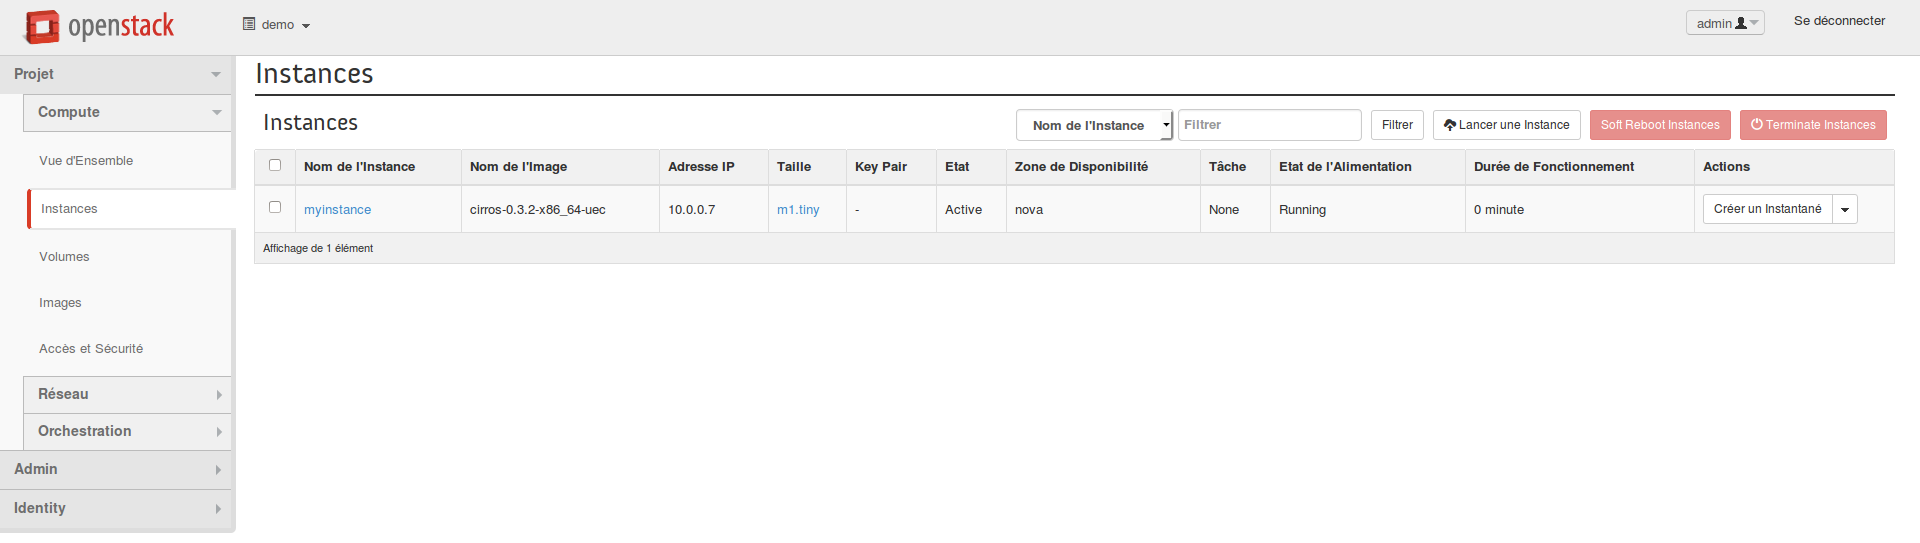
\includegraphics[width=\textwidth]{images/horizon.png}
  \end{frame}

